\nuovapagina

\vs(5)

{\normalsize \bf Criterio di complessit\a della curva}

\fbox{
\noindent
\begin{minipage}{16cm}
\vs(2)
\bfl
Problemi:
\ben
\im poter variare in modo automatico il numero dei punti di controllo
\im conservare la regolarit\a della curva
\een
\efl
\vs(5)
\end{minipage}
}

%--------------------------------------------------------------------------------------
\fbox{
\noindent
\begin{minipage}{16cm}
\vs(2)
\bfl
Soluzione:
\bi
\im ridistribuzione dei campioni della curva 
    \bi
    \im {\it reticolazione simpliciale} (o triangolazione) del piano
        [{\it Terzopoulos - anno}]
    \ei
    \vs(3)
    \centerline{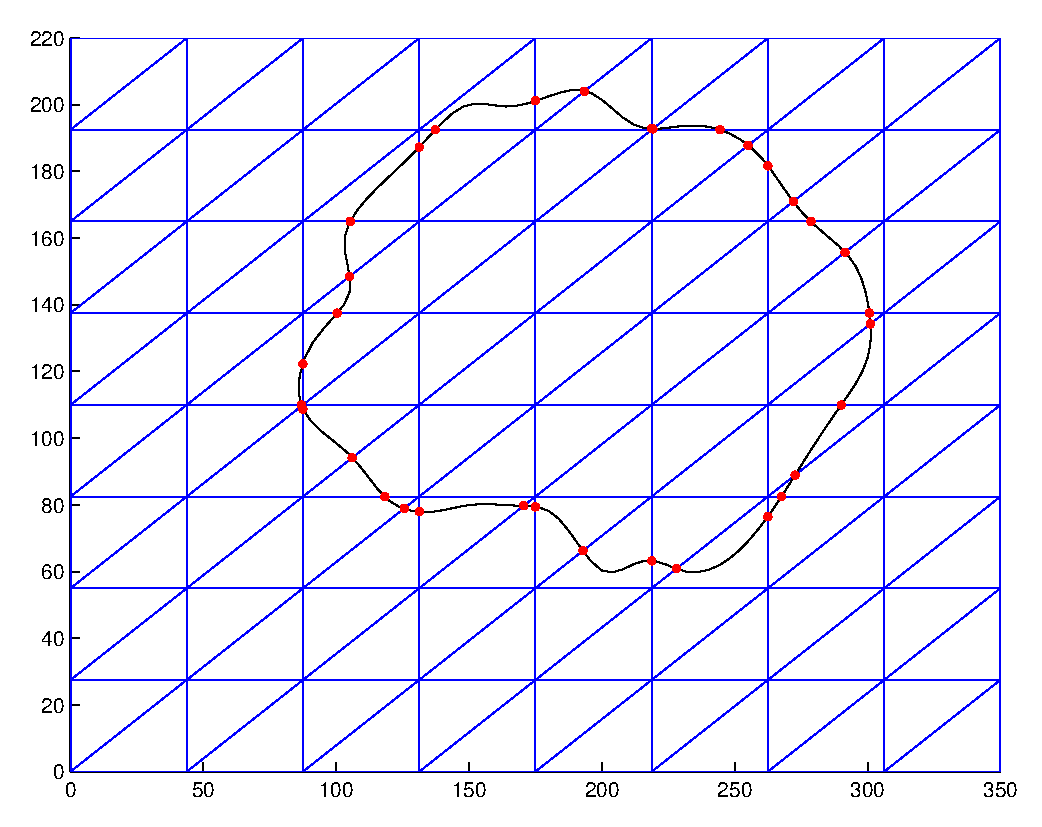
\psfig{file="./images/reticolo.eps",height=6cm,clip=}} 

\im 
    \bi
    \im a ciascun nuovo campione \e associata una "massa"
        $$
        \mu(i)\,=\,w_d\,d(i)\,+\,w_c\,c(i)
        $$
        che tiene conto della distanza dai due campioni precedente e successivo, $d$, e il
        grado di allineamento fra i tre, $c$.
    \im ogni nuovo span ha una "massa" totale inferiore a ${\cal M}$ prefissata
    \ei
\ei
\efl
\vs(5)
\end{minipage}
}
